% =====================================================================================
% Manuscrito para o European Journal of Operational Research (EJOR) -- classe elsarticle.
% STATUS (08/10/2026): rascunho NAO COMPILADO (sem LaTeX na maquina). Todo numero tem rastro em
% ../RASTREIO_NUMEROS.md. Itens "\pend{...}" bloqueiam a submissao.
% Autoria/declaracoes: preenchimento GENERICO (o pesquisador editara).
% =====================================================================================
\documentclass[preprint,12pt,authoryear]{elsarticle}

\usepackage{amsmath,amssymb}
\usepackage{booktabs}
\usepackage{multirow}
\usepackage{graphicx}
\usepackage{algorithm}
\usepackage{algpseudocode}
\usepackage{xcolor}
\usepackage[colorlinks=true,linkcolor=blue!50!black,citecolor=blue!50!black,urlcolor=blue!50!black]{hyperref}

\newcommand{\pend}[1]{\textcolor{red}{[PENDING: #1]}}   % marca bloqueadores de submissao
\newcommand{\pp}{\,pp}
\newcommand{\gap}{\mathrm{gap}}

\journal{European Journal of Operational Research}

\begin{document}

\begin{frontmatter}

\title{Does adaptive operator selection help? A controlled, pre-specified study of bandit-guided variable neighborhood search for the capacitated vehicle routing problem}

% ---- AUTORIA GENERICA: substituir ----
\author[inst1]{First Author\corref{cor1}}
\ead{first.author@example.org}
\author[inst1]{Second Author}
\cortext[cor1]{Corresponding author}
\affiliation[inst1]{organization={Department of [Department], [University]},
            city={[City]}, country={[Country]}}

\begin{abstract}
Machine-learning components are increasingly embedded in metaheuristics to select search operators, but their contribution is rarely separated from the search structure they are embedded in, and negative or null results are seldom reported with the same care as positive ones. We reproduce a recently published bandit-guided Variable Neighborhood Search (VNS) for the Capacitated Vehicle Routing Problem (CVRP), whose policy (HG-UCB) is reported to improve on plain VNS by 0.29 percentage points (pp), and test its learning component in four controlled studies on 74 CVRPLIB instances and 54 synthetic instances, under equal budgets, with hyperparameters tuned by one protocol for all policies, equivalence tests and a state-of-the-art reference. The published improvement is not reproduced: the faithful variant is about 0.9~pp worse than plain VNS, and our best variant ties with it. The cause we isolate is the reward scale: expressed in raw cost units, the reward saturates the policy's softmax, and normalizing it by solution cost removes a loss of 1.0--1.3~pp. With the reward corrected, no adaptive policy tested (HG-UCB, UCB1, $\varepsilon$-greedy, probability matching) beats uniform random selection, and benefits above about 0.16~pp are excluded by the data. What does improve results is search structure---stopping the inner loop at a local optimum (0.5--0.6~pp) and randomizing operator order (0.3--0.5~pp)---and the operator pool: adding five operators, including SWAP*, gains a further 0.5~pp. \pend{one sentence with the Study~4 results (tuned policies, tuned static mixture, synthetic validation).} A hybrid genetic search reference reaches a mean gap of 0.01--0.04\% on the same instances, so our conclusions concern the relative value of learning, not competitiveness. We provide the protocol, raw results and code to support similar audits of learning-guided heuristics.
\end{abstract}

\begin{highlights}
\item Published gain of bandit-guided VNS over plain VNS is not reproduced on CVRPLIB
\item Reward scale decides: raw-cost reward loses 1.0-1.3 pp to a normalized one
\item Adaptive selection never beats uniform random selection, in four controlled studies
\item Search structure and operator pool, not learning, drive gains of 0.3-0.8 pp
\item Open protocol: matched budgets, equivalence tests, HGS-CVRP and tuned baselines
\end{highlights}

\begin{keyword}
Routing \sep Metaheuristics \sep Variable neighborhood search \sep Adaptive operator selection \sep Multi-armed bandits \sep Reproducibility
\end{keyword}

\end{frontmatter}

\section{Introduction}\label{sec:intro}

Metaheuristics remain the workhorse for large routing problems, and a growing literature embeds machine-learning components in them to select search operators, tune parameters or guide moves \citep{karimimamaghan2022,bengio2021}. A common design is \emph{adaptive operator selection} (AOS): a policy observes the success of the operators applied so far and shifts the probability of choosing each one. Multi-armed-bandit policies are a popular choice for this role \citep{dacosta2008,fialho2010,lagos2024}, and adaptive weights are a standard ingredient of adaptive large neighborhood search \citep{ropke2006}. Newer proposals make operator selection a learned decision \citep{karimimamaghan2023,pei2023,xu2025}.

Whether such learning \emph{helps} is, however, a question that is rarely isolated. A learned policy is always evaluated inside a search with its own stopping rule, acceptance rule and operator order, and gains attributed to the policy may belong to the structure around it. The one meta-analytic estimate we know of is modest: across 25 implementations of adaptive large neighborhood search, the adaptive layer improved the objective by 0.14\% on average (95\% interval 0.06--0.21\%) \citep{turkes2021}.

This paper audits the learning component of one recent, representative method. \citet{kalatzantonakis2023} couple a variable neighborhood search (VNS) \citep{mladenovic1997,hansen2001} for the capacitated vehicle routing problem (CVRP) with a hybrid upper-confidence-bound and gradient-bandit policy (HG-UCB) and report that it improves on plain VNS by 0.29 percentage points (pp) of optimality gap on average over three benchmark sets. We ask five research questions.
\begin{description}
\item[RQ1 (reproduction)] Does the published improvement replicate, and what in the reward design determines the policy's behavior?
\item[RQ2 (structure)] How large are the effects of structural choices of the search (inner-loop termination, acceptance, operator order, operator pool) relative to learning?
\item[RQ3 (deterministic operators)] Under an equal budget, does adaptive selection beat non-adaptive (uniform) selection, and does the answer survive tuning, further policy families, larger instances, an efficient implementation of the costliest operator, a state-of-the-art solver and a positive control that shows the protocol can see a gain?
\item[RQ4 (stochastic operators)] With the stochastic operators of an adaptive large neighborhood search (CVRP and CVRP with time windows), does adaptive selection help, and is the gain adaptation or merely a good fixed weighting of the operators?
\item[RQ5 (generality)] Do the findings hold for another problem (the traveling salesman problem) and for one with new constraints (the CVRP with time windows), and where do they not?
\end{description}

We answer them with sixteen studies, each pre-specified in a dated research log before its data were produced, using 74 CVRP benchmark instances, 32 TSPLIB instances, 56 Solomon instances and 164 synthetic ones, ten random seeds (five on most synthetic sets), budgets measured in operator applications, in distance evaluations or in generations, paired nonparametric tests with Holm correction, bootstrap intervals, equivalence tests, a positive control and a state-of-the-art reference solver.

\paragraph{Contributions}
\begin{enumerate}
\item A reproduction of HG-UCB-guided VNS with its interpretation gaps documented. The published improvement is not reproduced, and we identify a failure mechanism: a reward in raw cost units saturates the policy's softmax, and normalizing it removes a loss of \num{s1a_hgucb_literal_hgucb_norm_800} to \num{s1a_hgucb_literal_hgucb_norm_4000} pp (Sections~\ref{sec:repro} and~\ref{sec:r1}).
\item Evidence, under matched budgets and with equivalence tests, that in the CVRP none of ten adaptive policy families beats uniform random selection with deterministic local-search operators (\num{u_n} contrasts, none better), and that the search structure (termination, operator order, operator pool, ruin and recreate) moves the gap far more (Sections~\ref{sec:r2} and~\ref{sec:r3}).
\item A positive control, repeated in three problems, showing that the protocol detects adaptive gains when they exist (Sections~\ref{sec:r4} and~\ref{sec:r6}).
\item A regularity across three routing problems: adaptive selection beats uniform selection where the pool contains costly operators that are not worth their cost (the larger pool is worse than the smaller one: the TSP, time windows, planted operators), and a non-adaptive design (a smaller pool, a descent ordered by cost, a tuned mixture or a fixed repair) obtains the same gain; in no setting is a policy significantly better than the best of these alternatives (the one policy that beats any fixed design, HG-UCB with time windows, beats a single repair that is no better than uniform selection, not the tuned mixture). A prospective test on eight further nested pools confirms the second statement without exception (\num{s15_foc_nb} of \num{s15_foc_n} contrasts against the fixed-order descent of the same pool favor a policy) but supports the first only as a tendency (Sections~\ref{sec:r5}--\ref{sec:r7}).
\item Practical guidance for choosing the selection layer of a local search, and an open, auditable protocol: pre-specification entries, exact-regression controls, operators validated by brute force, tables generated from raw results and recomputed independently (Section~\ref{sec:discussion}).
\end{enumerate}

\section{Related work}\label{sec:related}

\paragraph{Heuristics for the CVRP}
Variable neighborhood search systematically changes neighborhoods during descent and perturbation \citep{mladenovic1997,hansen2001}. For the CVRP, the strongest published heuristics are population-based or large-scale specialized methods; the hybrid genetic search of \citet{vidal2022}, with its SWAP* neighborhood, and the scalable local search of \citet{accorsi2021} define the current quality level, evaluated on the benchmark of \citet{uchoa2017} among others. We use the former only as a reference ceiling (Section~\ref{sec:ceiling}); the method we study is a lightweight VNS whose appeal is simplicity rather than absolute quality.

\paragraph{Adaptive operator selection}
Choosing which operator to apply from observed rewards is a multi-armed-bandit problem \citep{auer2002,suttonbarto2018}. In evolutionary computation, adaptive pursuit and probability matching \citep{thierens2005}, dynamic bandits \citep{dacosta2008} and a systematic analysis of bandit-based mechanisms \citep{fialho2010} established the framework; adaptive weights are also central to adaptive large neighborhood search \citep{ropke2006}, whose adaptive layer a meta-analysis quantified as a small average gain \citep{turkes2021}. Hyper-heuristics generalize the idea to selecting among low-level heuristics \citep{burke2013}; recent work includes bandit-based hyper-heuristics \citep{lagos2024}, Q-learning for operator selection in iterated greedy \citep{karimimamaghan2023}, correlation-assisted operator selection \citep{pei2023}, and a ranking of operators for routing neighborhoods \citep{voigt2025}. Neural methods that learn routing policies end to end \citep{kool2019} differ from operator-selection bandits in what is learned and when. Surveys of machine learning inside metaheuristics are given by \citet{karimimamaghan2022} and \citet{bengio2021}. These mechanisms are typically studied on operators, such as mutations, whose usefulness changes along the run; the best-improvement local-search operators of a VNS are deterministic and form a different setting, which is part of what we examine. Our study differs in its object (a specific published CVRP method), in its controls (matched non-adaptive baselines, a tuned static mixture, a factorial decomposition of the surrounding search) and in its inference (equivalence tests, not only significance tests).

\paragraph{Experimental methodology}
Matched budgets and honest baselines have been argued for decades \citep{hooker1995,barr1995}, and novelty without generalizable findings has been criticized \citep{sorensen2015}. We compare algorithms over instance sets with paired nonparametric tests and multiplicity correction \citep{wilcoxon1945,holm1979,derrac2011}, support claims of \emph{no difference} with equivalence testing \citep{lakens2017}, and tune all methods by one protocol, as in automatic configuration \citep{lopezibanez2016}.

\paragraph{Gap addressed}
To our knowledge, no study has isolated the learning component of a bandit-guided CVRP heuristic from its search structure under matched budgets, with all policies tuned by the same protocol and with equivalence testing. We do so for HG-UCB \citep{kalatzantonakis2023}, whose reproduction we report in full.

\section{Problem, reproduced method and reproduction fidelity}\label{sec:method}

\subsection{Problem and neighborhoods}
The CVRP asks for a set of routes, each starting and ending at a depot, that serves every customer exactly once, respects the vehicle capacity on each route and minimizes total distance. For sets A and B the number of routes must equal the number of vehicles of the best-known solution; for sets CMT and X it must be at least that number. Distances are rounded to the nearest integer for A, B and X and are real-valued for CMT, following the instance definitions.

Following \citet{kalatzantonakis2023}, the local search uses five best-improvement neighborhoods: 2-Opt and Move(1) inside a route, and Swap(1,1), Relocate(1,0) and Relocate(2,0) between routes. Each operator scans its entire neighborhood and applies the best improving move, so it is deterministic: repeating it on an unchanged solution cannot change it. Appendix~\ref{app:operators} gives the formal definitions, including the five additional operators of Study~3.

\subsection{The HG-UCB policy}\label{sec:hgucb}
Let $k$ be the number of operators and $\mathrm{H}_j$ a preference for operator $j$, with $q_j=\exp(\mathrm{H}_j)/\sum_l\exp(\mathrm{H}_l)$. HG-UCB selects operator $a_t$ by (i) trying every operator once (cold start); (ii) with probability $\varepsilon=0.1$, choosing uniformly from the pool $N_t=\{j:q_j\ge b_t\}$ ($b_t=0.2$); (iii) otherwise
\begin{equation}
a_t=\arg\max_{j\in N_t}\Big[q_j+C\sqrt{\tfrac{2\ln s_t}{n_j}}\Big],\qquad C=2,
\end{equation}
where $s_t$ counts selections and $n_j$ the applications of operator $j$. After applying operator $a_t$ with reward $r_t$ the preferences follow a gradient-bandit update,
\begin{equation}
\mathrm{H}_{a}\leftarrow \mathrm{H}_{a}+\alpha\,(r_t-\bar r_t)\,(\mathbb{1}[a=a_t]-q_a)\quad\forall a,
\end{equation}
with $\bar r_t$ the mean reward so far, and an ADWIN detector \citep{bifet2007} on the reward stream ($\delta=0.02$) resets the policy upon drift. The reward is
\begin{equation}
r^{+}=\rho\,|N_t|^{-1/n_{a_t}}\ \text{ if the move improves},\qquad r^{-}=-\tfrac12-2\,q_{a_t}^{\mathrm{prev}}\,|N_t|^{-1/n_{a_t}}\ \text{ otherwise},
\end{equation}
where $q^{\mathrm{prev}}$ is the operator's probability before the update and, in the published formulation, $\rho=c'-c''$ is the \emph{raw cost improvement} (cost of the reference solution minus cost of the new one). \emph{HG-UCB literal} denotes this formulation with $\alpha=5$, the value reported as best \citep{kalatzantonakis2023}.

\subsection{Interpretation gaps and our choices}\label{sec:gaps}
Reproducing the method from the published pseudocode required resolving four points, each documented in the research log:
\begin{enumerate}
\item \textbf{Unreachable stopping rule.} The inner loop stops when no improvement was found and $\max_j q_j<b_t$. With $k=5$ and $b_t=0.2$ this is impossible (a softmax of five values is never below $1/5$). We keep $b_t$ as published and add an explicit cap of 40 inner iterations (so the loop always runs to the cap).
\item \textbf{Scope of the reference solution.} The text can be read as keeping the shaken solution $x'$ fixed throughout the inner loop, or advancing it after each improvement. A fixed $x'$ prevents composing improvements from different operators within a step; with it our results are much worse (set A: 5.76\% against 4.21\%), so we use the progressive reading.
\item \textbf{Input of the drift detector.} The text says Q-values, the pseudocode the raw reward. We feed the raw reward; feeding Q-values worsened the gap in our tests.
\item \textbf{Acceptance rule.} The pseudocode does not state when the local-search result replaces the incumbent. For the classical GVNS baseline we accept only strict improvements of the best solution; in the bandit loop the result replaces the incumbent when it improves the shaken point (Section~\ref{sec:s2} varies this).
\end{enumerate}

\subsection{A reward-scale failure and its correction}\label{sec:norm}
With the raw-cost reward and $\alpha=5$, the softmax over preferences saturates: in an eight-instance diagnostic sample, 99.6\% of the iterations had $\max_j q_j>0.99$, so the probability filter and the exploration mechanism were effectively disabled. The range of $\alpha$ that avoids saturation depends on the instance's cost scale, since $r^{+}$ is in cost units (larger-cost X instances saturate at much smaller $\alpha$ than A or B). We therefore define a dimensionless reward by taking $\rho=(c'-c'')/c''$, which at the published $\alpha=5$ reduces saturation to 12.5\%. Unless stated otherwise, ``HG-UCB'' denotes this normalized reward with $\alpha=0.5$, the value that performed best in our diagnostic sweeps; since it was chosen on the same instances used for evaluation, Study~4 re-tunes it, together with all other policies, on disjoint instances.

\subsection{Reproduction fidelity}\label{sec:repro}
Table~\ref{tab:repro} compares our implementation, in the configuration closest to the published one (20 steps of 40 inner iterations, five seeds), with the numbers published for sets A, B and X \citep{kalatzantonakis2023}.

\begin{table}[t]
\caption{Reproduction fidelity: mean error (\%) over the instances of each set. Published values from the original study; ours from five seeds per instance. ``Literal'' uses the raw-cost reward and $\alpha=5$; ``normalized'' uses the dimensionless reward.}\label{tab:repro}
\centering\small
\begin{tabular}{lcccc}
\toprule
 & A & B & X & Mean of sets \\
\midrule
Published VNS & 2.040 & 1.832 & 6.291 & 3.388 \\
Published HG-UCB & 1.610 & 1.655 & 6.023 & 3.096 \\
\addlinespace
Ours: classical GVNS & 3.181 & 2.001 & 4.869 & 3.351 \\
Ours: HG-UCB literal, fixed $x'$ & 5.764 & 3.603 & 6.337 & 5.235 \\
Ours: HG-UCB literal, progressive $x'$ & 4.210 & 2.837 & 5.777 & 4.275 \\
Ours: HG-UCB normalized, $\alpha=5$ & 3.367 & 2.092 & 5.069 & 3.510 \\
Ours: HG-UCB normalized, $\alpha=0.5$ & 3.177 & 2.021 & 5.020 & 3.406 \\
\midrule
Published: HG-UCB $-$ VNS & $-$0.430 & $-$0.177 & $-$0.268 & $-$0.291 \\
Ours: literal (progressive) $-$ GVNS & $+$1.028 & $+$0.835 & $+$0.908 & $+$0.924 \\
Ours: normalized $\alpha=0.5$ $-$ GVNS & $-$0.004 & $+$0.020 & $+$0.151 & $+$0.056 \\
\bottomrule
\end{tabular}
\end{table}

Two observations qualify the reproduction. First, our classical GVNS agrees with the published VNS on the \emph{mean of the three sets} (3.351 against 3.388) but not set by set: it is worse on A (+1.14~pp) and B (+0.17~pp) and better on X ($-$1.42~pp). The published implementation is a cooperative parallel GVNS compiled with Cython, and details of operator order and acceptance are not fully specified, so the baseline is reproduced in aggregate, not instance by instance. Second, \emph{the published improvement of HG-UCB over VNS is not reproduced}: the configuration closest to the published one is 0.92~pp \emph{worse} than our GVNS, and with the corrected reward the difference is $+$0.06~pp, never the published $-$0.29~pp. This does not show that the published result is wrong; it shows that, with the implementation and acceptance rule we reconstructed from the text, the effect does not appear, and the differences listed above are candidate explanations that we did not test. We note also that the original study tuned its hyperparameters on three instances, two of which (B-n78-k10 and X-n120-k6) are among those later evaluated.

\section{Experimental design}\label{sec:design}

\subsection{Instances}
\paragraph{CVRPLIB.} We use 74 instances from CVRPLIB \citep{cvrplib}: set A (26 instances, 31--68 customers) and B (23, 30--77) with the classical definitions of Augerat et al.\ \citep{augerat1995}, set CMT (4, 50--120) of \citet{christofides1979}, and set X (21, 100--194) of \citet{uchoa2017}. The reference cost is the optimal or best-known value distributed with each instance.

\paragraph{Synthetic instances.}
To test generalization beyond CVRPLIB and to tune hyperparameters on instances disjoint from the evaluation set, we generate two synthetic sets with the X-instance generator of \citet{uchoa2017}, re-implemented as an in-process function and validated byte for byte against the official script (10 of 10 instances identical). \emph{Tuning set}: 24 instances (8 each with 50, 100 and 150 customers; seed 20261008). \emph{Validation set}: 30 instances (10 each with 100, 200 and 300 customers; seed 20261009). The combination of depot position, customer distribution, demand type and route length of each instance is sampled uniformly from the 378 combinations of the generator. The reference cost of each synthetic instance is the best of two runs of HGS-CVRP \citep{vidal2022} (seeds 1 and 2, 0.2~s per customer); it is not a proven optimum, and gaps are relative to it. As for set X, the number of routes of the reference solution is a lower bound.

\subsection{Budgets}\label{sec:budgets}
In Studies 1 and 2 the budget is the number of \emph{operator applications} $B\in\{800,4000\}$, counted by a wrapper around each neighborhood's best-improvement function; the shake does not count. The production configuration of the reproduced method (20 steps of 40 inner iterations) uses exactly 800 applications. With five similar operators this is a sound unit, but with operators whose cost differs by almost two orders of magnitude (Study~3) it would treat the most expensive operator as free. In Studies 3 and 4 the budget is therefore the number of \emph{distance evaluations} performed inside operators, $E_1=600\,n^2$ and $E_2=5E_1$ for $n$ customers, counted by a proxy of the instance that serves distances from a precomputed matrix. The count is deterministic given the seed, and the cost per evaluation is roughly constant (0.35--0.57~$\mu$s for $n$ between 53 and 195), so it tracks time without its noise on the heterogeneous cores of our machine. $E_1$ approximates the effort of 800 applications of the original pool; as a consistency check, the original pool with random order and local-optimum termination reaches 1.98\% at $E_2$ here and 1.94\% at $B=4000$ in Study~2. The check precedes each application; the application in progress completes, so a run overshoots its budget by at most the cost of one application (on average 0.03--0.6\%).

\subsection{Search structure}\label{sec:structure}
All arms share one generic loop (Algorithm~\ref{alg:loop}) parameterized by three structural factors---the operator \emph{selection policy}, the \emph{acceptance} rule and the inner-loop \emph{termination}---plus the pool. The initial solution is the Clarke--Wright savings solution repaired to satisfy the route-count constraint; the shake applies one random move from a randomly chosen original neighborhood and is identical across arms. Two code paths reproduce the earlier structures exactly (identical costs on all compared runs): fixed order/\emph{best}/LO reproduces the classical GVNS, and uniform/\emph{shaken}/F40 reproduces the original Algorithm~3 loop with uniform selection.

\begin{algorithm}[t]
\caption{Generic search loop. $B$ is the budget; policy $\pi$, acceptance $\in\{\textit{best},\textit{shaken}\}$, termination $\in\{\textrm{LO},\textrm{F40},\textrm{R}r\}$.}\label{alg:loop}
\begin{algorithmic}[1]
\State $x\gets$ initial solution; $x^*\gets x$
\While{budget not exhausted}
  \State $x'\gets \textsc{Shake}(x)$;\; $r\gets x'$;\; $F\gets\emptyset$;\; $m\gets 0$;\; $f\gets 0$
  \While{budget not exhausted \textbf{and} not stop}
    \State \textbf{stop if} LO: $|F|=k$;\; F40: $m=40$;\; R$r$: $f=r$
    \State choose operator $j\sim\pi$ (LO: among $\{1..k\}\setminus F$; else among all)
    \State apply best-improvement move of $j$ to $r$; update $\pi$ with the reward
    \If{improved} $r\gets$ new solution;\; $F\gets\emptyset$;\; $f\gets 0$ \Else\; $F\gets F\cup\{j\}$;\; $f\gets f+1$ \EndIf
    \State $m\gets m+1$
  \EndWhile
  \If{(\textit{best}: $c(r)<c(x^*)$) \textbf{or} (\textit{shaken}: $c(r)<c(x')$)} $x\gets r$;\; $x^*\gets r$ if $c(r)<c(x^*)$ \EndIf
\EndWhile
\State \Return $x^*$
\end{algorithmic}
\end{algorithm}

\subsection{Selection policies}\label{sec:policies}
\textbf{Uniform} (U) draws an operator uniformly; \textbf{fixed order} (FO) always takes the lowest-index allowed operator, which is the classical VND; \textbf{fixed order by cost} (FOC) cycles through a list ordered by increasing cost per application (fixed before the runs). \textbf{UCB1} \citep{auer2002} uses the reward normalized by the maximum observed, trying each operator once and then maximizing the normalized mean plus $C\sqrt{2\ln s/n_j}$ ($C=2$); \textbf{$\varepsilon$-greedy} uses the sample mean with $\varepsilon=0.1$; \textbf{probability matching} (PM) \citep{thierens2005} keeps an exponential moving average $Q_j\leftarrow Q_j+\gamma(r-Q_j)$ ($\gamma=0.1$) and selects with $p_j=p_{\min}+(1-kp_{\min})Q_j/\sum_lQ_l$ ($p_{\min}=0.05$); \textbf{HG-UCB} is described in Section~\ref{sec:hgucb}. Classical policies receive the relative improvement $(c'-c'')/c'$ on success and zero otherwise; HG-UCB receives its own reward. In Studies 3 and 4 the three learning policies use a \emph{cost-aware} reward: the success reward is multiplied by $\phi=\mathrm{clip}(\bar g/g,0.1,10)$, where $g$ is the distance evaluations of the application and $\bar g$ their running mean, so cheap successes are worth more; failures carry no cost information (a limitation we return to). The \textbf{static mixture} samples operators from a fixed distribution tuned offline (Study~4). Hyperparameter defaults come from the literature and from the original study (Appendix~\ref{app:hyper}); Study~4 tunes them.

\subsection{Studies}
Table~\ref{tab:studies} summarizes the four studies. Each was pre-specified (hypotheses, arms, tests and family size) in a dated research log before its data were produced (Appendix~\ref{app:prereg}).

\begin{table}[t]
\caption{Overview of the studies.}\label{tab:studies}
\centering\small
\begin{tabular}{p{1.4cm}p{3.6cm}p{2.8cm}p{3.6cm}p{2.0cm}}
\toprule
Study & Question & Structure and pool & Budget; instances; seeds & Confirmatory tests \\
\midrule
1 & Does the bandit beat chance? & Original loop (F40); 5 operators & $B\in\{800,4000\}$; 74 CVRPLIB; 10 & 12 (Holm) \\
2 & Where do differences come from? AOS inside VND? & Order $\times$ acceptance $\times$ termination; 5 operators & $B\in\{800,4000\}$; 74; 10 & 28 (Holm) \\
3 & Does a larger heterogeneous pool change it? & LO and R5; 10 operators & $E_1,E_2$; 74; 10 & 34 (Holm) \\
4 & Does tuning, a tuned static mixture or new instances change it? & R5; 10 operators & $E_1,E_2$; 74 and 30 synthetic; 10 and 5 & 14 and 6 (Holm) \\
\bottomrule
\end{tabular}
\end{table}

\subsection{Statistical protocol}
The unit of analysis is the instance: for each arm and instance the gap to the reference cost is averaged over the seeds (10 for CVRPLIB, 5 for the synthetic validation set), and arms are compared in pairs on the same instances. The primary test is the two-sided Wilcoxon signed-rank test \citep{wilcoxon1945}, because the paired differences are not normal (Shapiro--Wilk $p<0.05$ in 32 of 34 audited contrasts); omnibus comparisons use the Friedman test; multiplicity is controlled by the Holm procedure \citep{holm1979} over a family fixed before each study (Table~\ref{tab:studies}). Every comparison reports the mean paired difference in percentage points with a 95\% bootstrap confidence interval over instances (10\,000 resamples), wins, losses and ties. Because ``no significant difference'' is not evidence of equivalence, claims of no difference are supported by equivalence tests \citep{lakens2017}: two arms are equivalent within $\delta$ when the 90\% bootstrap interval of the mean difference lies within $(-\delta,+\delta)$ (a two one-sided tests procedure at 5\%), with $\delta=0.10$~pp as the primary margin (smaller than every confirmed structural effect, 0.13--0.8~pp) and 0.05, 0.15 and 0.20~pp as sensitivity. As a check on pseudoreplication, we also report 95\% intervals from a two-level bootstrap (instances, then seeds within instance, keeping the pairing by seed), and the minimum detectable effect at 80\% power, $2.8\,\mathrm{SD}_d/\sqrt{n}$ with $\mathrm{SD}_d$ the standard deviation of the paired instance differences. These robustness analyses were chosen after the confirmatory tests and are labeled as such.

\subsection{Verification}
Four controls precede the studies. (i) \emph{Exact regression} between code versions: each new version of the search loop must reproduce, cost for cost, the runs of the previous version under identical seeds (48 of 48 comparisons for the loop used in Study~2 after rewriting it; 8 of 8 and 6 of 6 for the cost-counting and instrumented paths). (ii) \emph{Operator validation}: the five additional operators were validated against an independent brute-force enumeration of their neighborhoods (1\,600 tests including infeasible-move and route-count cases), and a mutation test confirmed that the test can fail (a deliberately degraded SWAP* was detected in 29 of 40 cases). (iii) \emph{Accounting}: operator applications or distance evaluations match the budget in every run, and every returned solution is feasible (no infeasible run in any study). (iv) \emph{External reference}: HGS-CVRP solves all 74 instances in all runs with a feasible solution. \pend{independent recomputation of the headline gaps from raw costs by a script that shares no code with the analysis scripts.}

\subsection{Computing environment}
All runs used one laptop (Intel Core i5-12450H, 12 threads, 7.8~GB visible to the Linux subsystem), Windows 11 with an Ubuntu 26.04 LTS WSL2 guest, Python 3.14.4 (NumPy 2.5.3, SciPy 1.18.1, pandas 3.0.5, river 0.26.1 for ADWIN), and up to eleven parallel worker processes. HGS-CVRP (commit \texttt{1a92795}) was compiled with g++ 15.2.0 (\texttt{-O3}). Because budgets are in operator applications or distance evaluations, results do not depend on this hardware; wall-clock times are reported only descriptively.

\section{Results}\label{sec:results}
Differences are mean paired differences in percentage points (pp) of gap to the reference cost; a negative value favors the first-named arm. Brackets give 95\% bootstrap intervals over instances, $p$ values are Holm-adjusted over the family of the study, and ``wins'' and ``losses'' count the instances (74 CVRPLIB, or 30 synthetic; 25 and 30 in Study 7; the sets of Studies 8--12 are given in their sections) on which the first-named arm has the lower and the higher mean gap. Every number, table and figure of this section is generated from the raw per-run files by scripts (Section~\ref{sec:verification}). All runs of Studies 1--6 and 8--12 were feasible; Study~7 has \num{s7_ninv} exclusions (Section~\ref{sec:s7}).

\subsection{Study 1: does the bandit beat chance?}\label{sec:s1}
Study~1 keeps the original loop (40 inner applications per step) and compares HG-UCB with uniform selection, UCB1, $\varepsilon$-greedy, probability matching and the classical GVNS at a matched budget (Table~\ref{tab:s1}; all contrasts in Table~\stab{tab:s1tests}).

\begin{table}[t]
\caption{Study 1: mean gap (\%) over 74 instances, original loop.}\label{tab:s1}
\centering
\small
\begin{adjustbox}{max width=\linewidth}
\begin{tabular}{lcc}
\toprule
Policy & $B=800$ & $B=4000$ \\
\midrule
Classical GVNS (fixed-order VND) & 3.00 & 2.29 \\
Uniform & 3.41 & 2.72 \\
UCB1 & 3.39 & 2.73 \\
Probability matching & 3.47 & 2.80 \\
HG-UCB (normalized) & 3.47 & 2.83 \\
$\varepsilon$-greedy & 3.50 & 2.86 \\
HG-UCB literal & 4.43 & 4.14 \\
\bottomrule
\end{tabular}
\end{adjustbox}
\end{table}


HG-UCB does not beat uniform selection: \num{s1d_hgucb_norm_uniforme_800}~pp \num{s1ci_hgucb_norm_uniforme_800} at $B=800$ (adjusted $p=\num{s1p_hgucb_norm_uniforme_800}$) and \num{s1d_hgucb_norm_uniforme_4000}~pp \num{s1ci_hgucb_norm_uniforme_4000} at $B=4000$ (adjusted $p=\num{s1p_hgucb_norm_uniforme_4000}$); nor does it differ significantly from UCB1, $\varepsilon$-greedy or probability matching (adjusted $p\ge\num{s1_minp_others_4000}$). The literal variant is \num{s1a_hgucb_literal_hgucb_norm_800}~pp \num{s1ci_hgucb_literal_hgucb_norm_800} and \num{s1a_hgucb_literal_hgucb_norm_4000}~pp \num{s1ci_hgucb_literal_hgucb_norm_4000} worse than normalized HG-UCB, losing on \num{s1l_hgucb_literal_hgucb_norm_800} and \num{s1l_hgucb_literal_hgucb_norm_4000} of 74 instances: the reward scale, not the policy, produces a loss larger than any difference among policies. The classical GVNS has the lowest mean gap and is significantly better than HG-UCB (\num{s1a_hgucb_norm_gvns_classico_800}~pp \num{s1ci_hgucb_norm_gvns_classico_800} and \num{s1a_hgucb_norm_gvns_classico_4000}~pp \num{s1ci_hgucb_norm_gvns_classico_4000}; HG-UCB is worse on \num{s1l_hgucb_norm_gvns_classico_800} and \num{s1l_hgucb_norm_gvns_classico_4000} of 74 instances), a difference examined in Study~2. Of the 12 pre-specified tests, \num{s1_nsig} are significant.

An exploratory run at $B=20\,000$ (\num{sub_n} instances, 5 seeds; low power) shows the same pattern (HG-UCB minus uniform \num{sub_d_hu_20000}~pp, interval containing zero).

\subsection{Study 2: where do the differences come from?}\label{sec:s2}
A diagnostic explains why the original loop is inefficient (all 74 instances, 10 seeds, $B=800$; exploratory). On average \num{diag_ultima}\% of its 40 inner applications per step occur after the last improvement of that step, and \num{diag_otimo}\% occur after all five operators have failed on the current solution (by instance, \num{diag_otimo_min}--\num{diag_otimo_max}\%), when, since every neighborhood is deterministic, no further application can change the solution. The original loop performs \num{sh_f40_800} shakes within 800 applications; random order with local-optimum termination performs \num{sh_ubestlo_800} on average. Study~2 decomposes the structure by crossing operator \emph{order} (fixed or uniformly random), \emph{acceptance} (\textit{best} or \textit{shaken}) and inner-loop \emph{termination} (local optimum, LO, or 40 applications, F40) (Table~\ref{tab:s2a}; all contrasts in Table~\stab{tab:s2tests}).

\begin{table}[t]
\caption{Study 2A: mean gap (\%) over 74 instances by search structure (five operators).}\label{tab:s2a}
\centering
\small
\begin{adjustbox}{max width=\linewidth}
\begin{tabular}{lccc}
\toprule
Order / acceptance / termination & $B=800$ & $B=4000$ & Role \\
\midrule
Random / best / LO & 2.66 & 1.92 & best structure \\
Random / shaken / LO & 2.88 & 2.10 &  \\
Fixed / best / LO & 3.00 & 2.29 & classical GVNS \\
Fixed / shaken / LO & 3.18 & 2.58 &  \\
Random / best / F40 & 3.32 & 2.53 &  \\
Random / shaken / F40 & 3.41 & 2.72 & original loop, uniform \\
\bottomrule
\end{tabular}
\end{adjustbox}
\end{table}


\emph{Termination} is the dominant factor. Stopping at a local optimum instead of running 40 applications improves the gap by \num{g_term_abs}~pp across the two acceptance rules and two budgets (better on \num{g_term_w} of 74 instances; adjusted $p<10^{-4}$ in all four contrasts). \emph{Acceptance} contributes \num{g_acc_abs}~pp (all four contrasts significant, the weakest at adjusted $p=\num{s2p_C3_4000}$; descriptively the effect concentrates in set X, Table~\stab{tab:s2set}). Contrary to our pre-specified expectation, \emph{random order beats fixed order} by \num{g_ord_best_abs}~pp under \textit{best} acceptance and \num{g_ord_shaken_abs}~pp under \textit{shaken}, significantly at both budgets: the fixed order always restarts from 2-Opt, which then absorbs \num{s2_2opt_share_fixed_4000}--\num{s2_2opt_share_fixed_800}\% of all applications. Moving from the original loop to random order, \textit{best} acceptance and LO termination reduces the gap from \num{s2a_gap_uniforme_4000}\% to \num{s2a_gap_s2a_U_best_LO_4000}\% at $B=4000$ with no learning at all.

\paragraph{AOS inside the efficient structure}
In the best structure (\textit{best}/LO, selecting among operators not yet failed) we compare four adaptive policies with random order (rows D1--D4 of Table~\stab{tab:s2tests}). Probability matching ties with random order at both budgets, and UCB1 does at $B=800$ (\num{s2d_D1_800}~pp \num{s2ci_D1_800}); at $B=4000$ UCB1 is marginally worse (\num{s2d_D1_4000}~pp \num{s2ci_D1_4000}, adjusted $p=\num{s2p_D1_4000}$), a difference whose two-level interval \num{rb2_E2_4000_s2b_ucb1_s2a_U_best_LO} includes zero. $\varepsilon$-greedy and HG-UCB are significantly \emph{worse} at both budgets, a result that survives the two-level bootstrap (95\% intervals \num{rb2_E2_800_s2b_eps_greedy_s2a_U_best_LO} and \num{rb2_E2_4000_s2b_eps_greedy_s2a_U_best_LO} for $\varepsilon$-greedy; \num{rb2_E2_800_s2b_hgucb_norm_s2a_U_best_LO} and \num{rb2_E2_4000_s2b_hgucb_norm_s2a_U_best_LO} for HG-UCB). Adaptive policies are better than the classical fixed order by \num{g_vsfixed_abs}~pp, but this reflects the order effect above, not adaptation. Of the 28 pre-specified tests, \num{s2_nsig} are significant.

\subsection{Study 3: a larger, heterogeneous operator pool}\label{sec:s3}
With five similar deterministic operators there may be no room for adaptation. We therefore add 2-opt*, Or-opt (segments of 2--3), an intra-route swap, CROSS exchange (segments up to 3) and a naive SWAP* \citep{vidal2022}, for a pool of ten. The cost of an application differs by a factor of \num{eff_cost_ratio} across operators (mean \num{eff_cost_0}k distance evaluations for 2-Opt, \num{eff_cost_9}k for SWAP*; Table~\ref{tab:eff}) and the budget is therefore measured in distance evaluations (Section~\ref{sec:budgets}). We cross two stopping rules---LO, where adaptation can only reorder, and R5 (stop after five consecutive failures, sampling with replacement), where it can avoid costly useless operators---with five policies (Section~\ref{sec:policies}). Of the 34 pre-specified tests, \num{s3_nsig} are significant (\num{s3_nsig_E1} at $E_1$, \num{s3_nsig_E2} at $E_2$; Table~\ref{tab:s3}; all contrasts in Table~\stab{tab:s3tests}).

\begin{table}[t]
\caption{Study 3: mean gap (\%) over 74 instances (budgets $E_1$ and $E_2$); the last two rows use the original five operators with the same budget.}\label{tab:s3}
\centering
\small
\begin{adjustbox}{max width=\linewidth}
\begin{tabular}{lcc}
\toprule
Arm & $E_1$ & $E_2$ \\
\midrule
R5, UCB1 (cost-aware) & 2.10 & 1.33 \\
R5, uniform & 2.19 & 1.36 \\
R5, probability matching (cost-aware) & 2.19 & 1.40 \\
LO, uniform & 2.23 & 1.42 \\
LO, probability matching (cost-aware) & 2.25 & 1.43 \\
LO, UCB1 (cost-aware) & 2.26 & 1.45 \\
LO, HG-UCB (cost-aware) & 2.34 & 1.56 \\
R5, HG-UCB (cost-aware) & 2.15 & 1.56 \\
LO, fixed order by cost & 2.37 & 1.62 \\
\addlinespace
R5, fixed order by cost & 2.16 & 1.63 \\
Five operators, LO, uniform & 2.74 & 1.96 \\
Five operators, LO, fixed order & 2.99 & 2.30 \\
\bottomrule
\end{tabular}
\end{adjustbox}
\end{table}


\emph{The larger pool is the only large effect:} with the same stopping rule and random order, ten operators beat five by \num{s3a_T1_1}~pp \num{s3ci_T1_1} and \num{s3a_T1_5}~pp \num{s3ci_T1_5} at $E_1$ and $E_2$ (better on \num{s3w_T1_1} and \num{s3w_T1_5} of 74 instances; adjusted $p<10^{-4}$), in all four instance sets (Table~\stab{tab:s3set}). Random order again beats the classical fixed order for the original pool (\num{s3a_T3_1} and \num{s3a_T3_5}~pp). A fixed order \emph{by cost} is worse than random order with the large pool (\num{s3d_LO_FOCvsU_1} and \num{s3d_LO_FOCvsU_5}~pp under LO; \num{s3d_R5_FOCvsU_5}~pp under R5 at $E_2$). \emph{No adaptive policy beats uniform selection:} UCB1 and probability matching tie with it under both stopping rules and budgets, and HG-UCB is significantly worse at $E_2$ (\num{s3d_LO_hgucbcvsU_5}~pp \num{s3ci_LO_hgucbcvsU_5} under LO, \num{s3d_R5_hgucbcvsU_5}~pp \num{s3ci_R5_hgucbcvsU_5} under R5). UCB1 and probability matching do beat the fixed order by cost at $E_2$ (by \num{g_s3_vsfoc_abs}~pp), which reflects the weakness of that order. The cost-aware reward made no measurable difference to HG-UCB (\num{rbd_E3_1_s3_R5_hgucbc_s3_R5_hgucb_cego} and \num{rbd_E3_5_s3_R5_hgucbc_s3_R5_hgucb_cego}~pp at $E_1$ and $E_2$, intervals \num{rb1_E3_1_s3_R5_hgucbc_s3_R5_hgucb_cego} and \num{rb1_E3_5_s3_R5_hgucbc_s3_R5_hgucb_cego}). The stopping rule (R5 versus LO) has no detectable effect under random order (\num{s3d_T2_1} and \num{s3d_T2_5}~pp, not significant).

Uniform and adaptive policies spend \num{s3_swap_min}--\num{s3_swap_max}\% of their distance evaluations in SWAP* (the fixed order by cost, \num{s3_swap_foc_min}--\num{s3_swap_foc_max}\%), with HG-UCB concentrating the most (\num{s3_swap_hg_lo}\% under LO; Figure~S3 of the supplement). This concentration is a cost effect, not an efficiency one: SWAP* has the highest success rate per application (\num{eff_suc_9}\%) but the lowest relative gain per thousand distance evaluations, \num{eff_ratio} times below 2-Opt (Table~\ref{tab:eff}). Whether the benefit of the larger pool comes from the cheap or from the expensive additions is tested in Study~5.

\begin{table}[t]
\caption{Efficiency of each operator under uniform selection (R5, ten operators, $E_1$, 74 instances, 10 seeds): success rate per application, mean relative gain per success, mean cost per application (thousand distance evaluations) and relative gain (\%) per thousand distance evaluations, sorted by the last column.}\label{tab:eff}
\centering
\small
\begin{adjustbox}{max width=\linewidth}
\begin{tabular}{lcccc}
\toprule
Operator & Success (\%) & Gain/success (\%) & Cost (k eval.) & Gain per 1k eval. (\%) \\
\midrule
2-Opt & 37.3 & 1.10 & 1.1 & 0.364 \\
Move(1) & 38.7 & 1.06 & 1.9 & 0.219 \\
2-opt* & 24.3 & 1.45 & 1.8 & 0.192 \\
Swap-intra & 30.3 & 1.07 & 2.0 & 0.166 \\
Reloc(1,0) & 33.4 & 1.50 & 4.5 & 0.111 \\
Or-opt(2-3) & 37.2 & 1.23 & 5.2 & 0.088 \\
Reloc(2,0) & 10.6 & 2.34 & 3.8 & 0.065 \\
Swap(1,1) & 24.4 & 1.51 & 18.9 & 0.019 \\
CROSS & 21.5 & 1.48 & 24.7 & 0.013 \\
SWAP* & 40.0 & 1.55 & 70.9 & 0.009 \\
\bottomrule
\end{tabular}
\end{adjustbox}
\end{table}


\subsection{Study 4: tuned policies, a tuned static mixture and independent instances}\label{sec:s4}
Study~4 gives adaptation its best chance and measures the headroom. The hyperparameters of UCB1, probability matching and HG-UCB were tuned with one protocol (24 synthetic tuning instances disjoint from the evaluation instances, R5 structure at $E_1$, five seeds common to all configurations, grids of 5, 9 and 9 points; Section~7 of the online supplement), and a \emph{static mixture}---a fixed probability vector over the ten operators, with no learning---was tuned on the same instances by a $(1{+}4)$ evolution strategy (61 evaluations; weights in Table~\stab{tab:s4pesos}). Table~\stab{tab:s4config} lists the selected values. The gains of tuning on the tuning set are small for the three policies (\num{s4_tune_ucb1_d}\% to \num{s4_tune_ucb1_t}\% for UCB1, \num{s4_tune_pm_d}\% to \num{s4_tune_pm_t}\% for probability matching, \num{s4_tune_hgucb_d}\% to \num{s4_tune_hgucb_t}\% for HG-UCB) and of the order of the tuning noise: uniform selection implemented as an equal-weight static mixture differs from the uniform-selection arm by \num{s4_tune_noise}~pp on the same instances (different consumption of random numbers). The tuned static mixture, by contrast, improves the tuning-set gap from \num{s4_tune_static0}\% (equal weights) to \num{s4_tune_static_best}\%.



On the 74 CVRPLIB instances (Table~\stab{tab:s4tests}), \emph{no tuned policy beats uniform selection}: UCB1 \num{s4d_V1_1} and \num{s4d_V1_5}~pp, probability matching \num{s4d_V2_1} and \num{s4d_V2_5}~pp at $E_1$ and $E_2$ (no test significant), and tuned HG-UCB is significantly worse at $E_2$ (\num{s4d_V3_5}~pp \num{s4ci_V3_5}, adjusted $p=\num{s4p_V3_5}$). The improvement on the tuning set does not transfer: tuned UCB1 is no better than its default on CVRPLIB (\num{s4_gap_ucb1_t_1}\% against \num{s4_gap_ucb1_d_1}\% at $E_1$, \num{s4_gap_ucb1_t_5}\% against \num{s4_gap_ucb1_d_5}\% at $E_2$), as expected when the best of several noisy evaluations is selected. The \emph{static mixture} is at best marginally better than uniform selection: \num{s4d_V4_1}~pp \num{s4ci_V4_1} at $E_1$ (adjusted $p=\num{s4p_V4_1}$) and \num{s4d_V4_5}~pp \num{s4ci_V4_5} at $E_2$. Even with a distribution tuned offline on 24 instances, the gain over uniform selection is \num{s4a_V4_1}~pp at the smaller budget (not significant after correction) and null at the larger one, a benchmark for what a single global operator distribution can add. No tuned policy beats the static mixture (\num{s4d_V5_1}, \num{s4d_V6_1} and \num{s4d_V7_1}~pp at $E_1$ for UCB1, probability matching and HG-UCB; probability matching is significantly worse, adjusted $p=\num{s4p_V6_1}$). Of the 14 tests, \num{s4_nsig74} are significant, and in both the adaptive policy is the worse arm.

The learned mixture concentrates \num{s4_wp_2opt_pair}\% of its probability on 2-Opt and 2-opt*, two of the cheapest and most efficient operators, and only \num{s4_wp_expensive}\% on the three expensive ones, Swap(1,1), CROSS and SWAP* (Table~\stab{tab:s4pesos}), consistent with the per-evaluation efficiencies of Table~\ref{tab:eff}; it gives SWAP* only \num{s4_wp9}\% of its selections (although SWAP* absorbs \num{s4_static_swap_1}\% of its evaluations because of its cost), so the pool benefit does not require frequent use of the most expensive operator.

On the 30 synthetic validation instances (up to 300 customers, 5 seeds, $E_1$; Table~\stab{tab:s4val}) the pool effect replicates (\num{s4d_W1}~pp \num{s4ci_W1}, adjusted $p<10^{-4}$), whereas the effect of the fixed order by cost does not (\num{s4d_W2}~pp, adjusted $p=\num{s4p_W2}$) and no tuned policy differs from uniform selection (UCB1 \num{s4d_W3}, probability matching \num{s4d_W4}, HG-UCB \num{s4d_W5}~pp). The static mixture is \num{s4d_W6}~pp \num{s4ci_W6} from uniform selection (adjusted $p=\num{s4p_W6}$). Of the 6 tests, \num{s4_nsigval} is significant.

\subsection{Study 5: which operators explain the pool effect?}\label{sec:s5}
Table~\ref{tab:eff} suggests that the cheap operators are far more efficient than the expensive ones, so we expected the cheap additions to explain the benefit of the larger pool. Study~5 tests this with uniform selection on subsets of the pool (Table~\stab{tab:s5}): P8c adds 2-opt*, Or-opt and Swap-intra to the original five (P5), P7e adds CROSS and SWAP*, and P7c removes Swap(1,1), CROSS and SWAP* from the ten. \emph{The expectation is refuted:} the expensive pair is at least as valuable as the cheap trio. Adding the three cheap operators improves the gap by \num{g_s5_A1}~pp (range over the two stopping rules and the two budgets), whereas adding only CROSS and SWAP* improves it by \num{g_s5_A2}~pp and recovers \num{s5_rec_P7e_rng}\% of the effect of the full pool, against \num{s5_rec_P8c_rng}\% for the cheap trio (A1 and A2: all eight tests significant; Table~\stab{tab:s5tests}). The expensive operators still add value on top of the cheap ones (A3, \num{g_s5_A3}~pp, significant in \num{s5_A3_nsig} of 4 cases), removing Swap(1,1), CROSS and SWAP* from the ten operators costs \num{g_s5_A4}~pp (A4, significant in \num{s5_A4_nsig} of 4 cases), and even removing only Swap(1,1) from the eight-operator pool costs \num{g_s5_A5}~pp (A5, significant in \num{s5_A5_nsig} of 4 cases). Of the 20 pre-specified tests, \num{s5_nsig} are significant.


The operators that Table~\ref{tab:eff} ranks as least efficient therefore contribute substantially. Under uniform selection SWAP* absorbs \num{s5_p7e_swap_1}\% of the distance evaluations in P7e (CROSS \num{s5_p7e_cross_1}\%), and the tuned static mixture of Study~4 reaches a gap not significantly different from that of uniform selection over the ten operators while spending \num{s4_static_swap_1}\% of its evaluations on SWAP* instead of \num{s3_U_swap_1}\%. The per-evaluation efficiency measured under uniform selection thus understates the value of costly operators. A direct, exploratory diagnostic explains why: at \num{compl_n} local optima of the five original operators (74 instances, 3 seeds, 8 local optima each, reached by a fixed-order descent after a shake), one application of the best-improvement move of SWAP* finds an improvement in \num{compl_swapstar}\% of the cases and CROSS in \num{compl_cross}\%, against \num{compl_2opt}\% for 2-opt*, \num{compl_oropt}\% for Or-opt and \num{compl_swapintra}\% for Swap-intra; in \num{compl_so_caros}\% of the local optima only CROSS or SWAP* find an improvement, and in \num{compl_so_baratos}\% only the cheap added operators do. The expensive operators are complementary to the original ones: they improve solutions on which the cheap neighborhoods have failed.

\subsection{Study 6: further policy families and contextual policies}\label{sec:s6}
Study~6 asks whether the null results are specific to the four policy families examined so far. In the structure of Study~4 (R5, ten operators) and without tuning, we add EXP3, Thompson sampling, sliding-window UCB, adaptive pursuit, an efficiency UCB that charges the cost of every application (two exploration constants) and two contextual Thompson policies (Section~\ref{sec:policies}; Table~\ref{tab:s6}).

\inputopt{tab_s6}

\emph{No policy beats uniform selection:} none of the 16 pre-specified tests shows an improvement, and in \num{s6_nsig} of them the policy is significantly worse (Table~\ref{tab:s6}). EXP3 and sliding-window UCB are indistinguishable from uniform selection at both budgets (EXP3 \num{s6d_W1_1} and \num{s6d_W1_5}~pp, sliding-window UCB \num{s6d_W3_1} and \num{s6d_W3_5}~pp at $E_1$ and $E_2$). Thompson sampling and adaptive pursuit are worse (\num{s6d_W2_1} and \num{s6d_W2_5}~pp; \num{s6d_W4_1} and \num{s6d_W4_5}~pp), and so are the two contextual policies at $E_2$ (\num{s6d_W7_5} and \num{s6d_W8_5}~pp). The policy that charges the cost of every application is the worst of the study: with $C=1$ it is \num{s6d_W5_1} and \num{s6d_W5_5}~pp worse than uniform selection at $E_1$ and $E_2$, and with $C=2$ it is \num{s6d_W6_5}~pp worse at $E_2$. It does what it is designed to do, moving evaluations to cheap operators (at $E_2$, 2-Opt receives \num{s6_eff_2opt_5}\% of its evaluations and SWAP* \num{s6_eff_swap_5}\%, against \num{s3_U_2opt_5}\% and \num{s3_U_swap_5}\% under uniform selection), and, in line with Study~5, it loses because the expensive operators are worth more than their measured efficiency suggests. On the 30 synthetic validation instances (exploratory, $E_1$, no multiplicity correction) \num{s6v_nworse_raw} of the eight arms are nominally worse than uniform selection and one, sliding-window UCB, is nominally better (\num{s6vd_3}~pp \num{s6vci_3}, unadjusted $p=\num{s6vp_3}$); this difference does not survive a Holm correction over the eight comparisons (adjusted $p=\num{s6vph_3}$) and is not seen on CVRPLIB (\num{s6d_W3_1} and \num{s6d_W3_5}~pp).

\subsection{Study 7: adaptive move selection inside HGS-CVRP}\label{sec:s7}
Study~7 asks whether the null results hold inside a state-of-the-art local search (Section~\ref{sec:hgsaos}; Table~\ref{tab:s7}). They do, but the test is weak, because within HGS-CVRP the order in which the moves of a node pair are tried hardly matters. None of the 20 pre-specified tests is significant, the largest difference in absolute value is \num{s7_maxabs}~pp (\num{s7_maxabs_adapt}~pp for adaptive policies), and the original order does not differ significantly from the uniform random order either (on the synthetic instances at 250 generations it is \num{s7a_fixed_P2_250}~pp worse, interval \num{s7ci_fixed_P2_250}, whose lower limit is above zero, but the Wilcoxon test gives raw $p=\num{s7pr_fixed_P2_250}$). The minimum detectable effect at 80\% power is \num{s7_mde_med}~pp (median over the 20 tests). Of the 16 contrasts of adaptive policies at the primary checkpoints, \num{s7_neq} are equivalent to the random order within $\pm0.05$~pp, and so are all \num{s7_late_n} contrasts at 2000 and 4000 generations (exploratory). Including the \num{s7_ninv} runs excluded for violating the route-count bound of our convention (all on one instance, X-n195-k51) changes nothing (\num{s7_sens_nsig} significant tests). There is structure to learn, since the success rate per attempt varies by a factor of \num{s7_succ_ratio} across move types (from \num{s7_succ_2} to \num{s7_succ_4} improving moves per $10^4$ attempts under the random order), but because the first improving move is applied and a pair rarely admits several, ordering has little leverage, as a comment in the HGS-CVRP code notes. Budgets are matched in generations, not in CPU time: a generation takes \num{s7_cpu_fixed}~ms of CPU with the original order, \num{s7_cpu_unif}~ms with the uniform random order and \num{s7_cpu_ts}--\num{s7_cpu_hg}~ms with Thompson sampling to HG-UCB (probability matching, \num{s7_cpu_pm}~ms, suffers from floating-point underflow of its estimates, an implementation artifact). The original order is the fastest, so at equal CPU time it would beat every learned order, whereas the cost differences among the learned and random orders reflect our implementation. Because even randomizing the order changes so little, the study shows that nothing is gained at this decision point of HGS-CVRP; it is not evidence about other decision points of the solver.

\inputopt{tab_s7}

\subsection{Study 8: a positive control with planted useless operators}\label{sec:s8}
The null results above could reflect an insensitive protocol rather than the absence of exploitable structure. Study~8 (Section~\ref{sec:s8design}) adds four useless operators to the pool. Under uniform selection they absorb \num{s8_duds_D4x4_U}\% and \num{s8_duds_D4x8_U}\% of the distance evaluations and raise the gap by \num{s8_loss_D4x4}~pp and \num{s8_loss_D4x8}~pp (Table~\ref{tab:s8}). Of the 12 pre-specified tests, \num{s8_nsig} are significant, all in favor of the adaptive policy, so the protocol is not blind: Thompson sampling is \num{s8a_D4x8_ts}~pp better than uniform selection in the $8n^2$ pool (\num{s8ci_D4x8_ts}, adjusted $p=\num{s8p_D4x8_ts}$), the efficiency UCB \num{s8a_D4x8_eff}~pp (\num{s8ci_D4x8_eff}, $p=\num{s8p_D4x8_eff}$) and the cost-aware HG-UCB \num{s8a_D4x8_hgucbc}~pp ($p=\num{s8p_D4x8_hgucbc}$); in the $4n^2$ pool only UCB1 is significant (\num{s8a_D4x4_ucb1c}~pp, $p=\num{s8p_D4x4_ucb1c}$).

\begin{table}[t]
\caption{Study 8 (positive control): mean gap (\%) over 74 instances at $E_1$ in the clean pool of ten operators and in pools with four planted useless operators (each costing $4n^2$ or $8n^2$ distance evaluations and never improving); in parentheses, the difference from uniform selection \emph{in the same pool} in pp (* marks Holm-significance over the 12 confirmatory tests; clean-pool comparisons are exploratory).}\label{tab:s8}
\centering
\small
\begin{adjustbox}{max width=\linewidth}
\begin{tabular}{lccc}
\toprule
Policy & Clean pool & 4 useless, $4n^2$ & 4 useless, $8n^2$ \\
\midrule
Uniform selection & 2.19 & 2.55 & 2.72 \\
UCB1 (cost-aware) & 2.10 ($-$0.08) & 2.48 ($-$0.07*) & 2.67 ($-$0.05) \\
Probability matching (cost-aware) & 2.19 ($+$0.01) & 2.48 ($-$0.07) & 2.68 ($-$0.05) \\
HG-UCB (cost-aware) & 2.15 ($-$0.04) & 2.54 ($-$0.01) & 2.65 ($-$0.07*) \\
Thompson sampling & 2.32 ($+$0.14) & 2.43 ($-$0.12) & 2.51 ($-$0.22*) \\
EXP3 & 2.19 ($+$0.01) & 2.54 ($-$0.01) & 2.74 ($+$0.01) \\
Efficiency UCB & 2.48 ($+$0.29) & 2.50 ($-$0.05) & 2.56 ($-$0.16*) \\
\bottomrule
\end{tabular}
\end{adjustbox}
\end{table}


The policies differ sharply in how much of the planted loss they recover (exploratory; Table~\stab{tab:s8rec}). The efficiency UCB recovers \num{s8rec_D4x8_eff}\% of it in the $8n^2$ pool (interval \num{s8reci_D4x8_eff}) and Thompson sampling \num{s8rec_D4x8_ts}\% (\num{s8reci_D4x8_ts}), cutting the share of evaluations wasted on useless operators from \num{s8_duds_D4x8_U}\% to \num{s8_duds_D4x8_eff}\% and \num{s8_duds_D4x8_ts}\%; UCB1, probability matching, HG-UCB and EXP3 with default hyperparameters recover at most \num{s8rec_D4x8_pmc}\%, and keep spending \num{s8_duds_D4x8_hgucbc}--\num{s8_duds_D4x8_exp3}\% of the evaluations on the useless operators. For probability matching a structural reason is the exploration floor: with $p_{\min}=0.05$ and $k=10$ or 14 operators, 50\% or 70\% of the probability mass is reserved for uniform selection. Insurance has a premium: in the clean pool Thompson sampling and the efficiency UCB are significantly worse than uniform selection (\num{s8d_P10_ts} and \num{s8d_P10_eff}~pp, exploratory), and even the best policy in an inflated pool stays above uniform selection in the clean pool, so the best defense against a bad pool remains not to build one. The ceiling of what a policy can protect is itself small, because of diminishing returns of the budget: wasting \num{s8_duds_D4x8_U}\% of the evaluations costs only \num{s8_loss_D4x8}~pp.

\subsection{Study 9: adaptive selection in a stochastic large-neighborhood search}\label{sec:s9}
Study~9 (Section~\ref{sec:s9design}) is the first setting in which adaptive selection helps. The adaptive weights of Ropke and Pisinger are \num{s9prim_a}~pp better than uniform selection on the \num{s9_n_inst} instances (\num{s9prim_ci}; \num{s9prim_w} wins and \num{s9prim_l} losses; $p<10^{-4}$ in the single primary test), which lowers the mean gap from \num{s9_gap_U}\% to \num{s9_gap_RP}\% (Table~\ref{tab:s9}). Of the 12 secondary tests, \num{s9_nbetter} favor the adaptive policy after Holm correction: probability matching with the tuned $\gamma=0.05$ (\num{s9d_pm_X}~pp on set X and \num{s9d_pm_V}~pp on the synthetic set), EXP3 (\num{s9d_exp3_X} and \num{s9d_exp3_V}~pp) and HG-UCB on set X (\num{s9d_hgucb_X}~pp). UCB1 does not differ from uniform selection, and Thompson sampling and the efficiency UCB are much worse (\num{s9d_ts_V} and \num{s9d_eff_X}~pp on the sets where they are significant). The usage statistics show the mechanism: RP, UCB1 and probability matching move the repair choice to regret-2 (\num{s9_reg2_RP}\%, \num{s9_reg2_ucb1}\% and \num{s9_reg2_pm}\% of the repair choices, against \num{s9_reg2_U}\% under uniform selection), the operator that dominates the other two here. This heterogeneity of quality, which the best-improvement operators of the VNS do not have, is what the policies exploit, in line with the positive control of Study~8; the same two policies that were best against useless operators (Thompson sampling, the efficiency UCB) concentrate too early on the cheap or random operators and lose, so the choice of policy depends on the kind of heterogeneity.

\begin{table}[t]
\caption{Study 9 (ALNS with stochastic destroy and repair operators, $1500\,n^2$ distance evaluations): mean gap (\%) on the 21 instances of set X (ten seeds) and the 30 synthetic validation instances (five seeds); in parentheses, the difference from uniform selection in pp (* marks Holm-significance over the 12 secondary tests; for the adaptive weights, the primary test on the 51 instances is in the text and the per-set differences are exploratory). The last rows are VNS arms at the same budget.}\label{tab:s9}
\centering
\small
\begin{adjustbox}{max width=\linewidth}
\begin{tabular}{lcc}
\toprule
Policy & Set X & Synthetic validation \\
\midrule
Uniform selection & 1.48 & 1.86 \\
Adaptive weights (Ropke--Pisinger) & 1.24 ($-$0.24) & 1.42 ($-$0.44) \\
UCB1 & 1.74 ($+$0.26) & 2.20 ($+$0.34) \\
Probability matching & 1.15 ($-$0.33*) & 1.40 ($-$0.46*) \\
HG-UCB & 1.31 ($-$0.16*) & 1.60 ($-$0.26) \\
Thompson sampling & 2.63 ($+$1.16) & 3.04 ($+$1.18*) \\
EXP3 & 1.21 ($-$0.27*) & 1.52 ($-$0.34*) \\
Efficiency UCB & 3.45 ($+$1.97*) & 3.81 ($+$1.95*) \\
VNS, uniform selection (same budget) & 3.15 & 2.92 \\
VNS, static mixture (same budget) & 2.72 & 2.58 \\
\bottomrule
\end{tabular}
\end{adjustbox}
\end{table}


The search structure matters more than the selection layer: at the same budget, ALNS with uniform selection is better than VNS with uniform selection by \num{s9ta_vns_U_X} (set X) and \num{s9ta_vns_U_V}~pp (synthetic set), and better than VNS with the tuned static mixture by \num{s9ta_vns_static_X} and \num{s9ta_vns_static_V}~pp (Holm-adjusted $p\le0.002$ in the four tests). Two cautions apply. The gains of the adaptive policies are two to three times the average adaptive layer of the ALNS literature, and a fixed probability vector tuned offline might capture the same gain, since it can also learn that regret-2 is the best repair; this control is the object of Study~12 (Section~\ref{sec:s12}).

\subsection{Study 12: is the gain of the ALNS adaptation?}\label{sec:s12res}
It is not (Section~\ref{sec:s12}; Table~\ref{tab:s12}). A static mixture tuned offline (destroy probabilities \num{s12_wd_0}, \num{s12_wd_1}, \num{s12_wd_2} and \num{s12_wd_3}\% for random, worst, related and route removal; repair probabilities \num{s12_wr_0}, \num{s12_wr_1} and \num{s12_wr_2}\% for greedy, regret-2 and the cheap repair) is \num{s12a_static_U}~pp better than uniform selection (\num{s12ci_static_U}, adjusted $p<10^{-3}$), and the adaptive weights do not differ from it (\num{s12d_RP_static}~pp, \num{s12ci_RP_static}, adjusted $p=\num{s12p_RP_static}$); the static mixture captures \num{s12cap_static}\% of the gain of the adaptive weights over uniform selection (interval \num{s12capci_static}), and probability matching, the best adaptive arm, is \num{s12d_pm_static}~pp from it (adjusted $p=\num{s12p_pm_static}$). The simplest control does best: always using the regret-2 repair, with uniform destroy, is \num{s12a_reg2_U}~pp better than uniform selection and \num{s12a_RP_reg2}~pp \emph{better} than the adaptive weights (\num{s12ci_RP_reg2}; adjusted $p=\num{s12p_RP_reg2}$), the price of having to learn which repair is the best.

\begin{table}[t]
\caption{Study 12 (static control for the ALNS): mean gap (\%) on set X (21 instances), the synthetic validation set (30) and both (51), and the difference from uniform selection over the 51 instances in pp. The static mixture and the fixed repair are new arms; the other rows are the corresponding arms of Study 9 (same code, instances and seeds).}\label{tab:s12}
\centering
\small
\begin{adjustbox}{max width=\linewidth}
\begin{tabular}{lcccc}
\toprule
Policy & Set X & Synthetic & All & Difference \\
\midrule
Uniform selection & 1.48 & 1.86 & 1.70 \\
Static mixture (tuned offline) & 1.16 & 1.45 & 1.33 & $-$0.37 \\
Fixed repair: always regret-2 & 1.16 & 1.29 & 1.23 & $-$0.47 \\
Adaptive weights (Ropke--Pisinger) & 1.24 & 1.42 & 1.34 & $-$0.36 \\
Probability matching (tuned) & 1.15 & 1.40 & 1.30 & $-$0.40 \\
\bottomrule
\end{tabular}
\end{adjustbox}
\end{table}


The gain of Study~9 is therefore a gain from weighting the operators well, not from adapting during the run. What the adaptive policies provide is that discovery without tuning: the adaptive weights reach the level of the tuned mixture with no tuning run, whereas the mixture needed \num{s12_tune_runs} tuning runs (and a tuning gap of \num{s12_tune_gap}\% against \num{s12_tune_eq}\% for equal weights). This is consistent with the tuned static mixture of Study~4 and with Study~10, where no policy ever beat the best fixed configuration, and it sharpens the conclusion of the paper: adaptation recovers a good fixed configuration when none is available, but we found no setting in which it exceeds one.

\subsection{Study 10: larger instances}\label{sec:s10}
The pattern that motivated Study~10 does not replicate (Section~\ref{sec:s10design}; Table~\ref{tab:s10}). On the \num{s10_n_inst} new instances of 200 to 500 customers no mixture or policy is significantly better than uniform selection after correction: the mixture of Study~4 is \num{s10a_static_S}~pp better (\num{s10ci_static_S}; unadjusted $p=\num{s10pr_static_S}$, adjusted $p=\num{s10p_static_S}$) and the mixture tuned at this size \num{s10a_static_L}~pp better (\num{s10ci_static_L}; adjusted $p=\num{s10p_static_L}$), with a minimum detectable effect of \num{s10mde_static_L}--\num{s10mde_static_S}~pp at 80\% power; the three cost-aware online policies are within \num{s10a_ucb1c}~pp of uniform selection, and Thompson sampling and the efficiency UCB are significantly \emph{worse} (\num{s10d_ts} and \num{s10d_eff}~pp). The advantage of the mixtures does not grow with $n$: for the mixture tuned at this size it is \num{s10dn200_static_L}, \num{s10dn300_static_L}, \num{s10dn400_static_L} and \num{s10dn500_static_L}~pp at 200, 300, 400 and 500 customers (Spearman correlation with $n$ \num{s10rho_static_L}, $p=\num{s10rhop_static_L}$, the wrong sign for the hypothesis). The naive SWAP* absorbs \num{s10_swap_n200}--\num{s10_swap_n500}\% of the evaluations under uniform selection, so these instances are a demanding setting for any policy, yet tuning on them (gap \num{s10_tune_gap_eq}\% with equal weights, \num{s10_tune_gap_L}\% after the search) did not transfer. We conclude that the subgroup pattern of the earlier data was a selection effect, and that a mixture learned offline yields at best a few tenths of a point, with large variance.

\begin{table}[t]
\caption{Study 10: instances of 200 to 500 customers (20 synthetic validation instances, five seeds, $E_1$): mean gap (\%), mean paired difference from uniform selection in pp [95\% CI], unadjusted $p$ and Holm-adjusted $p$ over seven tests.}\label{tab:s10}
\centering
\small
\begin{adjustbox}{max width=\linewidth}
\begin{tabular}{lcccc}
\toprule
Policy & Gap & Difference & $p$ & $p$ (Holm) \\
\midrule
Uniform selection & 4.44 & & &  \\
Static mixture tuned at $n\le150$ (Study 4) & 4.04 & $-$0.40 [$-$0.69, $-$0.13] & 0.027 & 0.13 \\
Static mixture tuned at $n=200$--400 & 4.30 & $-$0.14 [$-$0.25, $-$0.04] & 0.030 & 0.13 \\
UCB1 (cost-aware) & 4.35 & $-$0.09 [$-$0.20, 0.02] & 0.143 & 0.43 \\
Probability matching (cost-aware) & 4.38 & $-$0.06 [$-$0.22, 0.11] & 0.498 & 0.52 \\
HG-UCB (cost-aware) & 4.41 & $-$0.03 [$-$0.13, 0.08] & 0.261 & 0.52 \\
Thompson sampling & 4.64 & $+$0.20 [0.10, 0.32] & 0.001 & 0.006 \\
Efficiency UCB & 4.68 & $+$0.24 [0.04, 0.43] & 0.008 & 0.050 \\
\bottomrule
\end{tabular}
\end{adjustbox}
\end{table}


\subsection{Study 11: do the results survive an efficient SWAP*?}\label{sec:s11}
They do (Section~\ref{sec:s11design}; Table~\ref{tab:s11}). Under uniform selection the efficient SWAP* costs \num{s11_cost_fast} thousand distance evaluations per application, against \num{eff_cost_9} for the naive one, and its share of the evaluations falls from \num{s11_swap_naive}\% in Study~3 to \num{s11_swap_E1}\% (CROSS now absorbs \num{s11_cross_E1}\%); it is still only the \num{s11_eff_rank}th of ten operators in gain per evaluation. Replacing the operator changes the gap of uniform selection by \num{s11vs3_d_E1}~pp at $E_1$ (better on \num{s11vs3_w_E1} of \num{s11_n74} instances) and \num{s11vs3_d_E2}~pp at $E_2$ (\num{s11vs3_w_E2} of \num{s11_n74}), a descriptive comparison with Study~3 under the same instances and seeds; on the 20 large synthetic instances the same replacement lowers the gap of uniform selection from \num{s10_gap_U}\% in Study~10 to \num{s11_gap_U_L}\%. As a regression control, the arm with the five original operators reproduces the corresponding arm of Study~5 cost for cost in \num{s11_reg_n} of \num{s11_reg_tot} runs.

None of the six online policies is significantly better than uniform selection in any of the 18 tests of the family, and \num{s11_nworse} are significantly worse: the efficiency UCB in the three scenarios (\num{s11d_eff_E1}, \num{s11d_eff_E2} and \num{s11d_eff_L}~pp) and cost-aware HG-UCB at $E_2$ (\num{s11d_hgucbc_E2}~pp, adjusted $p=\num{s11p_hgucbc_E2}$). Thompson sampling is worse by \num{s11d_ts_E1} and \num{s11d_ts_E2}~pp, but not significantly after correction (adjusted $p=\num{s11p_ts_E1}$ and \num{s11p_ts_E2}). The best online policy, cost-aware UCB1, is only \num{s11a_ucb1c_E1}, \num{s11a_ucb1c_E2} and \num{s11a_ucb1c_L}~pp better than uniform selection (adjusted $p=\num{s11p_ucb1c_E1}$ at $E_1$, unadjusted \num{s11pr_ucb1c_E1}), with minimum detectable effects of \num{s11mde_ucb1c_E2} to \num{s11mde_ucb1c_L}~pp. The mixture tuned for the efficient pool (\num{s11_w_0}\% 2-Opt, \num{s11_w_5}\% 2-opt*, \num{s11_w_9}\% SWAP*; tuning gap \num{s11_tune_gap}\% against \num{s11_tune_eq}\% with equal weights) is not significantly better than uniform selection either: \num{s11d_static_F_E1}~pp at $E_1$ and \num{s11d_static_F_E2}~pp at $E_2$ on the CVRPLIB instances, and \num{s11d_static_F_L}~pp on the large synthetic instances (\num{s11ci_static_F_L}; unadjusted $p=\num{s11pr_static_F_L}$, adjusted $p=\num{s11p_static_F_L}$, a minimum detectable effect of \num{s11mde_static_F_L}~pp), with no trend in $n$ (Spearman correlation \num{s11rho_static_F}, $p=\num{s11rhop_static_F}$).

\begin{table}[t]
\caption{Study 11 (efficient SWAP*): mean gap (\%) and, in parentheses, the paired difference from uniform selection in pp and its Holm-adjusted $p$ (21 tests), on the 74 CVRPLIB instances at $E_1$ and $E_2$ and on the 20 large synthetic instances at $E_1$; the last row is the pool of the five original operators under the same structure.}\label{tab:s11}
\centering
\small
\begin{adjustbox}{max width=\linewidth}
\begin{tabular}{lccc}
\toprule
Policy & CVRPLIB $E_1$ & CVRPLIB $E_2$ & Large synthetic $E_1$ \\
\midrule
Uniform selection & 1.89 & 1.18 & 3.87 \\
UCB1 (cost-aware) & 1.81 ($-$0.07; 0.50) & 1.12 ($-$0.05; 1.0) & 3.76 ($-$0.11; 1.0) \\
Probability matching (cost-aware) & 1.91 ($+$0.02; 1.0) & 1.20 ($+$0.02; 1.0) & 3.72 ($-$0.15; 1.0) \\
HG-UCB (cost-aware) & 1.93 ($+$0.04; 1.0) & 1.36 ($+$0.18; 0.0002) & 3.79 ($-$0.08; 1.0) \\
Thompson sampling & 1.96 ($+$0.08; 0.25) & 1.33 ($+$0.15; 0.054) & 3.78 ($-$0.09; 1.0) \\
EXP3 & 1.92 ($+$0.03; 1.0) & 1.17 (0.00; 1.0) & 3.83 ($-$0.04; 1.0) \\
Efficiency UCB & 2.34 ($+$0.46; \ensuremath{<10^{-4}}) & 2.14 ($+$0.96; \ensuremath{<10^{-4}}) & 4.34 ($+$0.47; 0.015) \\
Static mixture tuned for the efficient pool & 1.81 ($-$0.07; 1.0) & 1.21 ($+$0.03; 1.0) & 3.55 ($-$0.32; 1.0) \\
Uniform, five original operators (P5) & 2.91 & 2.11 & --- \\
\bottomrule
\end{tabular}
\end{adjustbox}
\end{table}


The effect of the pool, in contrast, persists and grows: uniform selection over the ten operators is \num{s11a_set_E1} and \num{s11a_set_E2}~pp better than over the five original ones at $E_1$ and $E_2$ (\num{s11ci_set_E1} and \num{s11ci_set_E2}; wins and losses \num{s11w_set_E1}/\num{s11l_set_E1} and \num{s11w_set_E2}/\num{s11l_set_E2}; adjusted $p<10^{-3}$), against \num{s11vs3_set_E1} and \num{s11vs3_set_E2}~pp with the naive operator (descriptive comparison with the arms of Studies 3 and 5). The central results therefore do not depend on the cost of the naive SWAP*: the absence of gains from selection and the effect of the pool hold with the efficient operator, which still lacks the polar-sector restriction of HGS-CVRP.

\subsection{Robustness of the null results: equivalence, power and pseudoreplication}\label{sec:robust}
We audited the \num{eq_n} contrasts of Studies 1--4 and 6 that compare a policy (or the static mixture) with its baseline (Figure~\ref{fig:forest} shows the \num{eq_n_aos} contrasts of adaptive policies); the choice of contrasts and margins is post hoc and the confirmatory tests above are unchanged. At $\delta=0.10$~pp only \num{eq_010} of \num{eq_n} contrasts are equivalent (\num{eq_015} at 0.15~pp, \num{eq_020} at 0.20~pp), mostly UCB1 and probability matching against uniform selection; HG-UCB is never equivalent to uniform selection at $\pm0.10$~pp. The most favorable lower limit of a 90\% interval among the contrasts of adaptive policies is $-\num{eq_best_lo90}$~pp, so gains over uniform selection above about \num{eq_best_lo90}~pp are excluded by our data (under the assumptions of the interval). The minimum detectable effect at 80\% power is \num{mde_med}~pp (median). Two-level bootstrap intervals are \num{rb_wider_min}--\num{rb_wider_max}\% wider (median \num{rb_wider_med}\%) and change the reading of marginal contrasts (HG-UCB versus uniform in the original loop at $B=4000$ no longer excludes zero: \num{rb2_E1_4000_hgucb_norm_uniforme}), while the findings we emphasize retain intervals excluding zero. The standard error of a ten-seed mean is about \num{seed_se_E1}~pp (\num{var_dentro_E1}\% of the variance of a single run's gap is between seeds), comparable to the effects studied, which is why we pair by instance and seed.

\begin{figure}[!htbp]
\centering
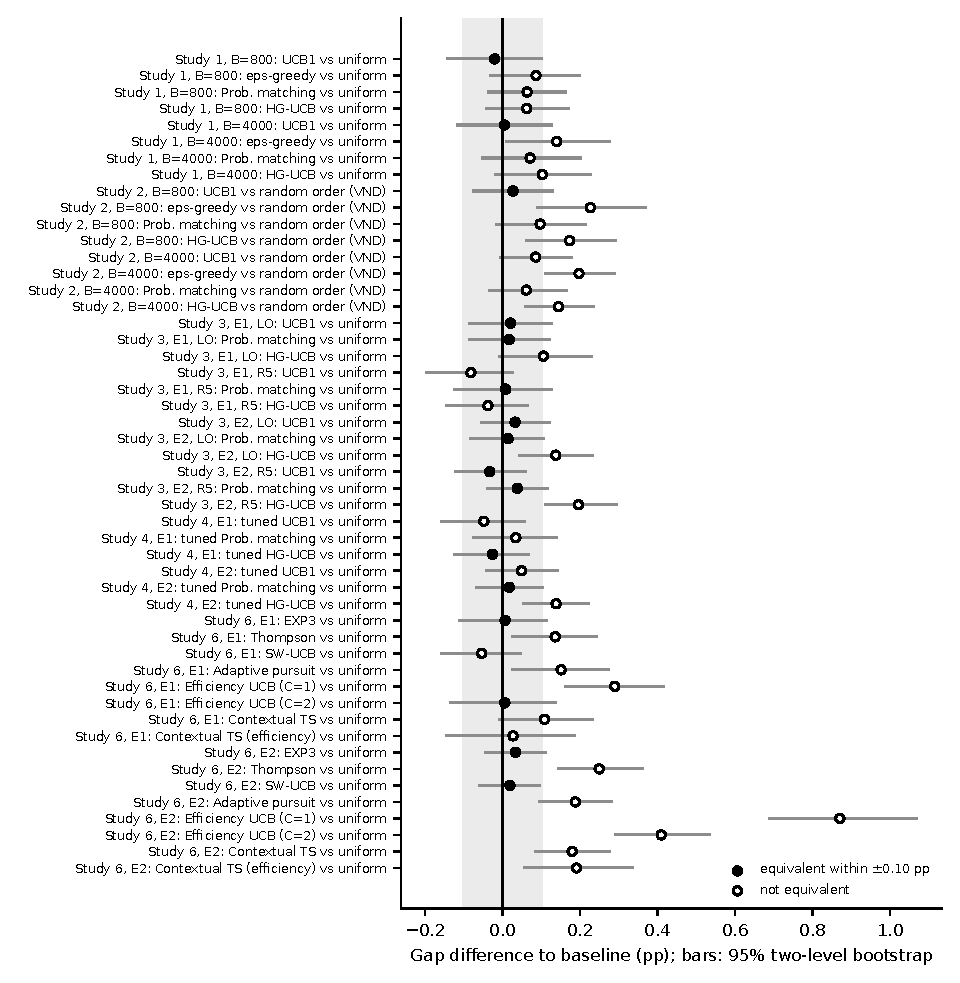
\includegraphics[width=0.9\linewidth]{fig_forest.pdf}
\caption{Equivalence audit: gap difference between each adaptive policy and its baseline in Studies 1--4 and 6. Filled markers: 90\% interval inside $\pm0.10$~pp (equivalent). Bars: 95\% two-level bootstrap intervals.}\label{fig:forest}
\end{figure}

\subsection{Reference ceiling and context}\label{sec:ceiling}
For context, HGS-CVRP \citep{vidal2022}, given the same wall-clock budget as our VNS (\num{hgs_matched_t_min}--\num{hgs_matched_t_max}~s per instance), reaches a mean gap of \num{hgs_matched}\% on the 74 instances, and \num{hgs_n01}\% with 0.1~s per customer, against \num{vns_gap_min}--\num{vns_gap_max}\% for the (non-literal) VNS variants studied here. Part of this distance is implementation language (C++ against Python), so we claim no ranking, only that no variant studied is competitive with the state of the art. An attention-based constructive model \citep{kool2019} used zero-shot reaches a mean gap of \num{kool_gap}\% over the 74 instances when the route-count constraint is ignored (\num{kool_gap_strict}\% on the \num{kool_nstrict} instances that satisfy it).
\section{Discussion}\label{sec:discussion}

\paragraph{What the evidence says about learning}
Across the original loop, a standard VND, a ten-operator pool, tuned policies, further policy families (including one that learns the gain per distance evaluation) and the move order of HGS-CVRP (Studies 1--4, 6 and 7), no adaptive policy outperformed uniform random selection (none of \num{u_n} confirmatory contrasts shows a significant improvement, whereas \num{u_worse} show the policy significantly worse), and the policy under study, HG-UCB, was significantly worse than chance in \num{u_hg_worse} of its \num{u_hg_n} contrasts. The equivalence audit rules out gains of adaptation above about \num{eq_best_lo90}~pp, and a static operator mixture tuned offline gains at most \num{s4a_V4_1}~pp over uniform selection at the smaller budget and nothing at the larger one, so there is little headroom for a policy to capture by learning a global preference among these operators. The size of the bound is of the order of the average gain of the adaptive layer in a meta-analysis of adaptive large neighborhood search (an improvement of the objective by 0.14\%, \citealp{turkes2021}, which is, up to the normalization by the reference cost, a difference of 0.14~pp in gap), whereas termination, operator order and the operator pool changed the gap by \num{g_struct_lo} to \num{g_struct_hi}~pp, \num{g_struct_x_lo} to \num{g_struct_x_hi} times more.

\paragraph{Why adaptation has so little to gain here}
Four mechanisms are consistent with our data. (i) \emph{Deterministic operators and local optima.} Each operator applies its best improving move, so once all operators have failed on a solution nothing more can be learned or gained; in the original loop \num{diag_ultima}\% of the applications of a step follow its last improvement and \num{diag_otimo}\% follow the point at which all five operators have failed, which also left a policy only the first few applications of each step to influence. (ii) \emph{Weak and sparse signal.} Most applications fail and the successes are small relative improvements, so the learned policies stay close to uniform (HG-UCB uses each of the five operators \num{s2_hg_use_min}--\num{s2_hg_use_max}\% of the time). (iii) \emph{Cost, not success, separates the operators.} In the ten-operator pool the operators differ by a factor of \num{eff_ratio} in gain per distance evaluation (Table~\ref{tab:eff}), but a distribution tuned on 24 instances to exploit this gains little over uniform selection (Study~4), and a patience stopping rule does not significantly improve on stopping at a local optimum (Study~3). (iv) \emph{Cost of failures.} The cost-aware reward of Studies 3 and 4 credits cheap successes but not the cost of failures; the policy of Study~6 that does charge them is the worst of all (\num{s6d_W5_5}~pp at $E_2$ with $C=1$), because expensive operators are worth more than their efficiency suggests (Study~5).

\paragraph{What does improve the results}
Stopping the inner loop at local optima, randomizing the operator order and enlarging the operator pool changed the gap by more than any policy. Study~5 shows that the pool effect has no single source: the three cheap added operators and the two expensive ones each recover a large part of it, the expensive pair more (\num{s5_rec_P7e_rng}\% against \num{s5_rec_P8c_rng}\%), although they are the least efficient per distance evaluation under uniform selection (Table~\ref{tab:eff}); they are what finds improvements at the local optima of the original operators (Section~\ref{sec:s5}). Efficiency measured in that way is therefore not a safe guide for pruning an operator pool, whereas an ablation of the pool itself is. In applications where the operators are cheap and similar, the practical implication is that the simplest option, a VND with random operator order that stops at local optima, is a strong default, and that effort is better spent on the operator pool and on its cost profile than on the selection layer.

\paragraph{Implications for the design and evaluation of learning-guided heuristics}
Four practices follow. First, \emph{include a matched non-adaptive control}: without it, the policies of Study~2 would appear to improve on the classical fixed order by \num{g_vsfixed_abs}~pp, a gain that belongs to randomization. Second, \emph{check the scale of the reward}, since a reward in cost units can turn a nominally adaptive method into one that is worse than chance. Third, \emph{ablate the search structure and the operator pool}, which moved the gap by more than any policy. Fourth, \emph{report equivalence, not only non-significance}, and add a \emph{tuned static mixture} to bound what adaptation can capture.

\paragraph{Relation to the original study}
We do not claim that the published improvement is wrong: our reconstruction differs from the original implementation in aspects that the pseudocode leaves open (acceptance rule, operator order, cooperative parallel search, compiled code), and our baseline agrees with the published one only on the mean of the three sets. We can say that the effect is not reproduced under a faithful-as-possible reconstruction, that the reward as published is scale-dependent, and that the improvement attributed to learning is smaller than the effects of structure in our experiments.

\subsection{Limitations}
\begin{itemize}
\item \emph{Platform.} Most of our searches are a Python VNS with deterministic best-improvement operators and gaps of \num{vns_gap_min}--\num{vns_gap_max}\%, against \num{hgs_n01}--\num{hgs_matched}\% for a hybrid genetic search. Study~7 tests adaptive ordering of the node-pair moves inside HGS-CVRP, with a binary reward, batched index updates and SWAP* left outside the policy's control; because even randomizing that order changes the gap by at most \num{s7_maxabs}~pp, it is a weak test, and adaptive choice among whole neighborhoods or among the genetic operators of a state-of-the-art solver is not tested. We claim no ranking or competitiveness.
\item \emph{Policies and operators.} Ten adaptive policy families and a static mixture, on two operator pools from one family of neighborhoods. Contextual policies were tested only with the previous operator and its outcome as context; richer solution features, stochastic operators and other reward definitions may behave differently, and the new families of Study~6 and the policies of Study~7 were not tuned.
\item \emph{Tuning.} Policies were tuned on a modest grid with five seeds at one structure and budget, with unequal effort across families, and the tuning noise (\num{s4_tune_noise}~pp) is of the order of the gains of tuning; a larger tuning budget or an automatic configuration procedure \citep{lopezibanez2016} might yield a better adaptive policy.
\item \emph{Instances.} 74 CVRPLIB instances with up to 194 customers and 54 synthetic ones with up to 300; synthetic reference costs are the best of two HGS runs, not proven optima. Only the CVRP is studied.
\item \emph{Inference.} Tests use instance means, so seed variance is summarized, not modeled; two-level intervals address this only partially. The equivalence margin (except in Study~7) and the robustness analyses were chosen after the confirmatory tests.
\item \emph{Pre-specification.} Hypotheses were written in a dated research log before each study ran, but without an external registry; version-control timestamps exist for Study~4 (commit \texttt{ef82cdc}), Study~6 (\texttt{02e58d3}, extended by \texttt{b3d4add}) and Study~7 (\texttt{8a06b17}), each before its data; the entry of Study~5 was committed after its runs had started, and Studies 1--3 rest on the log alone.
\item \emph{Reproduction.} The published implementation could not be obtained; the reproduction rests on the published description and four documented interpretation choices.
\end{itemize}

\section{Conclusions}\label{sec:conclusions}
Auditing a published bandit-guided VNS for the CVRP, we found that its reported improvement is not reproduced, that the reward as published can reduce it to worse-than-random behavior, and that, once the reward is normalized, none of the adaptive policies tested beats uniform random selection: not in the original loop, inside a standard VND, with a heterogeneous operator pool, after tuning, nor with further bandit families and a policy that learns the gain per distance evaluation, nor for the move order inside the local search of a state-of-the-art genetic algorithm, a weak test because that order barely matters. The gains came from elsewhere: stopping the inner loop at local optima, randomizing operator order and enlarging the operator pool. Both cheap and expensive added operators contribute to the pool effect, the expensive ones more than their efficiency per evaluation suggests. For operations research the lesson is methodological as much as algorithmic: the four practices listed above should precede any claim about the contribution of a learned component. Natural extensions are testing adaptation at other levels of state-of-the-art solvers, richer contextual policies, and other routing problems; our protocol, data and code are provided to support them.


% ------------------------------- Declarations (GENERICAS) -------------------------------
\section*{CRediT authorship contribution statement}
\textbf{First Author:} Conceptualization, Methodology, Software, Validation, Formal analysis, Investigation, Data curation, Writing -- original draft, Visualization. \textbf{Second Author:} Conceptualization, Supervision, Writing -- review \& editing. \pend{confirm the contributions of each author.}

\section*{Declaration of generative AI and AI-assisted technologies in the writing process}
During the preparation of this work the authors used Claude (Anthropic) for code development, scripting of statistical analyses, verification of references against primary sources, and drafting and editing of text, and Gemini (Google) for independent second opinions on ambiguous readings of the reproduced method. After using these tools, the authors reviewed and edited the content as needed and take full responsibility for the content of the publication. \pend{authors to confirm the extent of their own supervision and edit this statement.}

\section*{Declaration of competing interest}
The authors declare that they have no known competing financial interests or personal relationships that could have appeared to influence the work reported in this paper. \pend{confirm.}

\section*{Funding}
\pend{funding sources, or an explicit statement that there were none.}

\section*{Data and code availability}
The protocol (pre-specification entries), instances (CVRPLIB subsets and the synthetic sets with their HGS-CVRP reference solutions), raw per-run results, analysis scripts and the research log are available at \pend{persistent repository DOI, to be minted at submission (Zenodo or equivalent)}. Third-party code (HGS-CVRP) is available from its authors under the MIT license.

\section*{Acknowledgements}
\pend{acknowledgements, if any.}

\appendix
\section{Operators}\label{app:operators}
\setcounter{table}{0}
Let a solution be a set of routes; $d(\cdot,\cdot)$ is the (symmetric) distance, $0$ the depot, $q$ the demand and $Q$ the capacity. Every operator evaluates its whole neighborhood and applies the move with the most negative cost change $\Delta$ if $\Delta<0$; moves that violate capacity, or that would empty a route when this would violate the route-count constraint, are excluded. Costs change only through the edges listed.
\begin{description}
\item[2-Opt] In a route $(\dots,a,b,\dots,c,d,\dots)$ reverse the segment from $b$ to $c$: $\Delta=d(a,c)+d(b,d)-d(a,b)-d(c,d)$.
\item[Move(1)] Move one customer $u$ with neighbors $p,s$ to another position between $x,y$ of the same route: $\Delta=d(x,u)+d(u,y)-d(x,y)-d(p,u)-d(u,s)+d(p,s)$.
\item[Swap(1,1)] Exchange customers $u\in R_1$ and $v\in R_2$ between routes (each takes the other's place).
\item[Relocate(1,0)] Move one customer from route $R_1$ to any position of route $R_2$.
\item[Relocate(2,0)] Move two consecutive customers, in either orientation, from $R_1$ to any position of $R_2$.
\item[2-opt*] For routes $A$, $B$ and cut points $i,j$, exchange tails: $A'=A_{<i}\,B_{\ge j}$, $B'=B_{<j}\,A_{\ge i}$.
\item[Or-opt(2--3)] Move a segment of two or three consecutive customers, with or without inversion, to another position of the same route.
\item[Swap-intra] Exchange two customers of the same route.
\item[CROSS($\le3$)] Exchange a segment of $l_A$ customers of $A$ with one of $l_B$ customers of $B$, $l_A,l_B\in\{1,2,3\}$, $\max(l_A,l_B)\ge2$, preserving segment orientation.
\item[SWAP*] \citep{vidal2022} Exchange $u\in A$ and $v\in B$, reinserting $u$ at the best position of $B\setminus\{v\}$ and $v$ at the best position of $A\setminus\{u\}$ (not necessarily each other's place). Our version evaluates all pairs without the polar-sector restriction or top-three insertion lists of the original, so it is slower.
\end{description}
All ten operators were validated against an independent enumeration of their neighborhoods (Section~\ref{sec:verification}). The shake applies one random move from a randomly chosen original neighborhood, accepted even if it worsens the solution.

\section{Hyperparameters}\label{app:hyper}
\setcounter{table}{0}
\begin{table}[h]
\caption{Policy hyperparameters. Defaults are used in Studies 1--3 and 6; Study~4 tunes the first four families (default in bold in the grids).}\label{tab:hyper}
\centering\small
\begin{adjustbox}{max width=\linewidth}
\begin{tabular}{lll}
\toprule
Policy & Default & Study 4 grid \\
\midrule
UCB1 & $C=2$ & $C\in\{0.1,0.3,1,\mathbf{2},4\}$ \\
Probability matching & $\gamma=0.1$, $p_{\min}=0.05$ & $\gamma\in\{0.05,\mathbf{0.1},0.3\}\times p_{\min}\in\{0.02,\mathbf{0.05},0.1\}$ \\
HG-UCB & $\alpha=0.5$, $C=2$, $\varepsilon=0.1$, $b_t=0.2$, ADWIN $\delta=0.02$ & $\alpha\in\{0.1,\mathbf{0.5},2\}\times C\in\{1,\mathbf{2},4\}$ \\
Static mixture & uniform & $\theta\in\mathbb{R}^{10}$, $(1{+}4)$ evolution strategy, 15 generations \\
$\varepsilon$-greedy & $\varepsilon=0.1$ & not tuned \\
EXP3 & $\gamma=0.1$ & not tuned (Study 6) \\
Thompson sampling & Beta(1,1) prior & not tuned (Study 6) \\
Sliding-window UCB & window 200, $\xi=0.6$ & not tuned (Study 6) \\
Adaptive pursuit & $\alpha=\beta=0.1$, $p_{\min}=0.05$ & not tuned (Study 6) \\
Efficiency UCB & $C=1$ and $C=2$ & not tuned (Study 6) \\
Contextual Thompson sampling & prior strength $k_0=5$, 21 contexts & not tuned (Study 6) \\
Patience (R5) & $r=5$ & not tuned \\
Inner cap (F40) & 40 & not tuned \\
Cost-aware factor & $\mathrm{clip}(\bar g/g,0.1,10)$ & not tuned \\
\bottomrule
\end{tabular}
\end{adjustbox}
\end{table}


\bibliographystyle{elsarticle-harv}
\bibliography{../refs}

\end{document}
